\chapter {Descripción y Módulos de Ambienta2MX}
  \section {¿Qué y para qué es Ambienta2MX?}
    \paragraph {\underline{Ambienta2MX} es el nombre de la plataforma que formará parte de una macro solución orientada a la estandarización de metadatos que el INEGI y otras instituciones públicas.}
    \paragraph{Actualmente no existe un estándar de datos geográficos a nivel nacional. Han existido aproximaciones mediante concursos que instituciones públicas como el INEGI ha publicado, o simplemente han existido propuestas que han brindado una solución incompleta a la unión y manejo de información geográfica, geodésica, hidrográfica, climática, topográfica, etc.}
    \paragraph{\underline{Ambienta2MX} toma parte de todo el problema y propone una infraestructura lógica para afrontar la estandarización de variables ambientales y algunos índices de contaminación. Esta información actualmente se encuentra en formatos muy rudimentarios como textos planos sin algún protocolo o formato de interpretación.}
    \paragraph{Sistemas semejantes, por ejemplo, el \textbf{Servicio Meteorológico Nacional} carece de algún recurso del cual se puedan realizar consultas que no sea mediante su portal web, esto trae problemas directos de compatibilidad con otros sitemas. Un caso semejante tenemos con la información que la \textbf{Conagua} maneja en sus centrales meteorológicas a lo largo del país, los datos que brindan se actualizan de forma periodica y el único medio de acceso es a través de una página de internet que devuelve archivos en formato de texto u hojas de cálculo.}
    \paragraph{Los impedimentos antes mencionados conllevan a situaciones tan triviales como la consulta de datos para algúna región o punto específico del territorio nacional, al existir diversas fuentes no es posible tener un compendio del cual tomar la información que más nos convenga. Si a este problema se le añade que los datos carecen de un estandar, llegamos al punto en el que intentar manipular o tratar los datos se vuelve una tarea complicada y en exceso tediosa.}
    \paragraph{Considerando dichos problemas \underline{Ambienta2MX}, propone un estandar de datos climáticos tomando como referencia diversas fuentes y adaptando los tipos de datos a tecnologías y tendencias actuales, brindando así una mayor portabilidad y simplicidad en la consulta de información.}
  \newpage
  \section{Diagrama de Ambienta2MX}
    \paragraph{\underline{Ambienta2MX} constará de varios módulos que trabajarán de forma conjunta para satisfacer la necesidad de tener un estandar y un repositorio de datos climáticos a nivel nacional.}
    \paragraph{Al brindar un sistema modularizado, se genera de forma directa un impacto en el proceso de análisis, desarolló e intengración. Éste tipo de modelo describe de una forma sencilla los componentes necesarios para solventar la demanda a la que se encontrará sometida la plataforma.}
    \paragraph{A continuación se muestra el diagrama a bloques de \underline{Ambienta2MX}, todos los módulos, recursos y bases de datos serán descritos de forma posterior.}
  \newpage
  	\begin{landscape}
	  	\begin{figure}[h!]
	    \caption{Módulos y estructura de Ambienta2MX}
	  	\centering
		  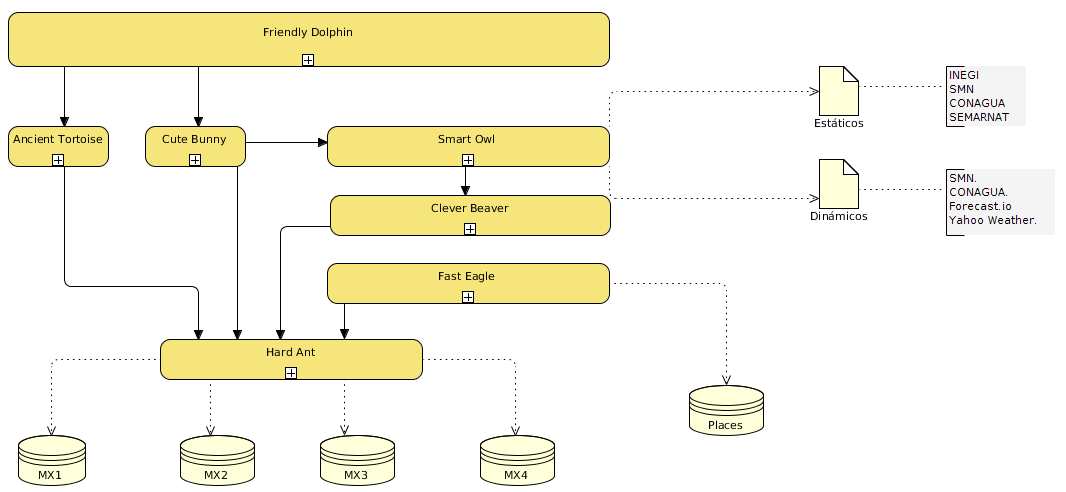
\includegraphics[width=22.5cm,height=12cm]{./images/DiagramaAmbienta2MX.png}
		\end{figure}
  	\end{landscape}
  \newpage
    \paragraph{Cómo se apreciar en el diagrama, además de los gestores de bases de datos, \underline{Ambienta2MX} se encuentra dividido en siete módulos básicos:}
    \begin{itemize}
		\item Friendy Dolphin.
		\item Ancient Tortoise.
		\item Cute Bunny.
		\item Smart Owl.
		\item Clever Beaver.
		\item Fast Eagle.
		\item Hard Ant.
	\end{itemize}
    \paragraph{En el mismo diagrama se pueden observar las fuentes que proporcionarán la información ya sea a un nivel estático, por ejemplo, carta climática anual de algún municipio del territorio nacional; o bien, recursos que se actualizan de forma periodica como son los datos que provee el Servicio Meteorológico Nacional.}
    \paragraph{Se condieran cinco bases de datos, \emph{MX1, MX2, MX3, MX4, Places}. Todas las bases del tipo MX contarán con la información de variables ambientales así también de los índices de contaminación de las zonas que conforman al territorio nacional.}
    \paragraph{Para el caso de \emph{Places}, la base será usada como un macro índice cartográfico del territorio nacional, es decir, esta base será la referencia a nivel latitud, longitud y altitud para ubicar los datos que requieran ser procesados.}
    \paragraph{Todas las bases se encontrarán funcionando bajo un modelo de base de datos documental teniendo una alimentación bajo demanda, es decir, el contenido gestionado irá aumentando conforme las éstos vayan siendo solicitados.}